\documentclass[11pt]{article}
\usepackage{amssymb,amsmath,amsthm,graphicx}
\usepackage{fancyhdr}

\def\shownotes{1}   % set 1 for version with author notes
                    % set 0 for no notes



%uncomment to get hyperlinks
%\usepackage{hyperref}

%%%%%%%%%%%%%%%%%%%%%%%%%%%%%%%%%%%%%%%%%%%%%%%%%%%%%%%%%%%%%%
%Some macros (you can ignore everything until "end of macros")

\topmargin 0pt \advance \topmargin by -\headheight \advance
\topmargin by -\headsep

\textheight 8.9in

\oddsidemargin 0pt \evensidemargin \oddsidemargin \marginparwidth
0.5in

\textwidth 6.5in

%%%%%%

\providecommand{\vs}{vs. }
\providecommand{\ie}{\emph{i.e.,} }
\providecommand{\eg}{\emph{e.g.,} }
\providecommand{\cf}{\emph{cf.,} }
\providecommand{\etc}{\emph{etc.} }

\newcommand{\getsr}{\gets_{\mbox{\tiny R}}}
\newcommand{\bits}{\{0,1\}}
\newcommand{\bit}{\{0,1\}}
\newcommand{\Ex}{\mathbb{E}}
\newcommand{\eqdef}{\stackrel{def}{=}}
\newcommand{\To}{\rightarrow}
\newcommand{\e}{\epsilon}
\newcommand{\R}{\mathbb{R}}
\newcommand{\N}{\mathbb{N}}
\newcommand{\Gen}{\mathsf{Gen}}
\newcommand{\Enc}{\mathsf{Enc}}
\newcommand{\Dec}{\mathsf{Dec}}
\newcommand{\Sign}{\mathsf{Sign}}
\newcommand{\Ver}{\mathsf{Ver}}

\providecommand{\mypara}[1]{\smallskip\noindent\emph{#1} }
\providecommand{\myparab}[1]{\smallskip\noindent\textbf{#1} }
\providecommand{\myparasc}[1]{\smallskip\noindent\textsc{#1} }
\providecommand{\para}{\smallskip\noindent}


\newtheorem{theorem}{Theorem}
\theoremstyle{definition}
\newtheorem{ex}{Exercise}
\newtheorem{definition}{Definition}

%%%%%%%  Author Notes %%%%%%%d
%
\ifnum\shownotes=1
\newcommand{\authnote}[2]{{ $\ll$\textsf{\footnotesize #1 notes: #2}$\gg$}}
\else
\newcommand{\authnote}[2]{}
\fi
\newcommand{\Snote}[1]{{\authnote{Solution}{#1}}}
\newcommand{\Inote}[1]{{\authnote{Solution}{#1}}}
\newcommand{\Ichanged}[1]{{\authnote{Changed}{#1}}}
%%%%%%%%%%%%%%%%%%%%%%%%%%%%%%%%%

\newcommand{\VAR}{\mathrm{VAR}}



% end of macros
%%%%%%%%%%%%%%%%%%%%%%%%%%%%%%%%%%%%%%%%%%%%%%%%%%%%%%%%%%%%%%


% page counting, header/footer
\usepackage{fancyhdr}
\pagestyle{fancy}
\lhead{\footnotesize \parbox{11cm}{CS350, Boston University, Fall 2015} }
\rhead{Erik Brakke}
\renewcommand{\headheight}{24pt}

\begin{document}

\title{Homework 10}
\author{Erik Brakke}
\maketitle

\thispagestyle{fancy}


\section*{Answer 1}
Assumption: you can combine two separate datasets in map reduce (i.e. if one map produces A and another map then reduce produces B in the form (k,vs), then I can just combine A + B)\\

See q1.py for a python implementation

$D$ is the initial dataset where the key is the category, and the value is a list of people who like the category
First, we want to compute the intersection of every pair\\
$Map(D): \text{ For every combination of people in this key } emit((p1, p2), category)$ only if $p1 < p2$\\
$Reduce(k, vs): return (k, vs)$\\
This will first emit tuples where the key is the two people who like the same category, and the value is the category itself\\
The reduce will condense this down so for every pair of people that had something in common, there is now a list of things they like\\
We will call this data set $I$\\
\newline
Next we need the union of everyone's interests.  To do so we will first map everyone to a single key so we can get all combinations of people\\
$Map(D): \text{ for every person and category } emit(*, (p, c))$\\
$Reduce(k, vs): return (k, vs)$\\
After this reduce, we will have one data entry with the key $*$ and the value will be one entry for every person and category of the form (person, category).  We will call this $CI$\\
\newline
Now we want the cross product of all of the people and the things they like.\\
$Map(CI) = \text{ for every pair of persons where p1 < p2 } emit((p1[0],p2[0]), [p1[1], p2[2]])$\\
$Reduce(k, vs) = return (k, set(vs))$ (we cast set just to make sure there are no duplicates)\\
In this, we first emit every possible pair of people and every possible thing they like.  The 0 element of the person is what the person ID is, and the 1st element is a category they like.  Now we have things that are keyed on a pair of people and two things they like\\
The reduce then produces every pair of people and a list of things they like (the union).  We will call this $U$\\
\newline
Now we can compute the intersection / union\\
First we must combine our intersection and union together into a dataset called $B$\\
Now we just need to reduce again\\
$Map(B) = emit(k, v)$ (We don't need to expand on what we already have)\\
$Reduce(k, vs) = return(k, sorted(vs))$\\
We do a noop map and then for the reduce we sort the values by the length of the list\\
This is because we know the intersection will be $\le$ the union, so we just want to know which is first\\
Now we can compute the values we want\\
$Map(B) = emit(k, v)$\\
$Reduce(k, vs) = return(k, 0 if len(vs[0]) == 1 else  len(vs[0][0]) / len(vs[0][1]))$\\
This will just emit 0 if they didn't share anything in common, otherwise it will compute the coefficient.


\section*{Answer 2}
See code in src folder and data in AsData.txt\\
To achieve this, first I counted the number of occurences of each AS.  The reason behind this, is if the AS appear once, that meant that it was connected to another AS, thus its degree count should be incremented.  I emitted values of (AS, 1) where the AS is the key.  Then I reduced by summing up all of the degrees of each AS.  Next, I took this data and emitted the key as the count and the value 1.  Then reduced by key to get the degree, and then number of ASes having that degree.\\
This is the histogram on the ASes and their degrees.  It is split into 150 buckets.  From this we can see that most ASes are on the lower end (the max being a degree of 2), but the range of degrees is quite large (up to about 6000)\\
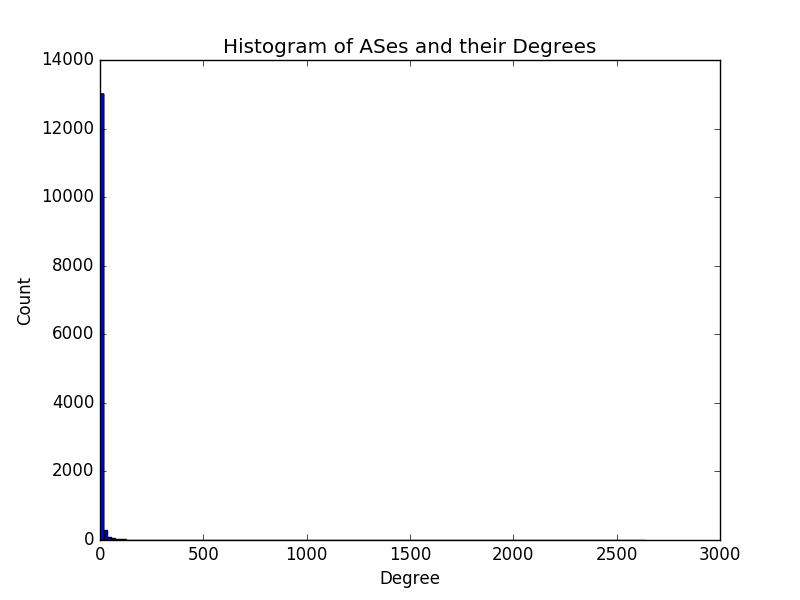
\includegraphics[scale=0.5]{hist}

\section*{Answer 3}
\begin{enumerate}
  \item[a.] See src for code.  For this I read in every word and split it up into letters.  Then for every letter, if it was a vowel, I incremented the count of vowels by one.  After reading all the letters, I emitted (count, 1) to show that there was an occurence of that many vowels appearnig.  Then I just reduced by summing these up to get the number of occurrences for each vowel count\\

  \item[b.]
\end{enumerate}

\section*{Answer 4}
\begin{enumerate}
  \item[a.] Using the same technique as above, I was able to generate a similar output\\
  See the aws\_screenshot\_q4a.png for proof of running on AWS.  THe output is also in q4a\_1.txt and q4a\_2.txt

  \item[b.]
\end{enumerate}


\end{document}
